\section{Results}

 \frame{\sectionpage}

\begin{frame}{Estimation I: Exogenous Treatment}
\only<1->{
    \small
    \begin{equation*}
        E_{ms} = \alpha + \textcolor{orange}{\beta}A_{ms} + X_{ms}\gamma + \nu_s+ \epsilon_{ms}
    \end{equation*}
}

\uncover<1->{
    \begin{table}[h!]
        \footnotesize
        \begin{center}
            \label{tab:result1}
            \begin{tabular}{lcccc}
            
            & \multicolumn{2}{c}{All incumbent mayors} & & Those ran \\
            & (1) & (2) & & (3) \\
            \hline
            Preelection audit (1/0) & \textcolor<2-3>{orange}{-0.036} & \textcolor<2-4>{orange}{0.036} & & \textcolor<2,4>{orange}{-0.059} \\
             & \textcolor<2-3>{orange}{(0.053)} & \textcolor<2-4>{orange}{(0.052)} & & \textcolor<2,4>{orange}{(0.065)}\\
             Observations & 373 & 373 &  & 263\\
             $R^2$ & 0.05 & 0.17 & & 0.22\\
             State FEs & Yes & Yes & & Yes\\
             Municipal controls & \textcolor<3>{orange}{No} & \textcolor<3>{orange}{Yes} & & Yes \\
             Mayoral controls & \textcolor<3>{orange}{No} & \textcolor<3>{orange}{Yes} & & Yes
            \end{tabular}
        \end{center}
        \end{table}

    {\footnotesize \textbf{\color{orange} Note:} Hereafter, robust standard errors are displayed in parenthesis, significant levels: 99\%(**), 95\%(*), 90\%(+).}
    }
    
\end{frame}

\begin{frame}{Estimation I: Exogenous Treatment}
    \only<1->{
    \small
    \begin{equation*}
        E_{ms} = \alpha + \textcolor{orange}{\beta}A_{ms} + X_{ms}\gamma + \nu_s+ \epsilon_{ms}
    \end{equation*}
}

\uncover<1->{
    \begin{table}[h!]
        \footnotesize
        \begin{center}
            \label{tab:result2}
            \begin{tabular}{lccccc}
            
            \multicolumn{6}{c}{Only mayors ran for reelection}\\
            \hline
            & Pr(reelection) & Vote share & Win margin & $\Delta$vote share & $\Delta$win margin \\
            & (3) & (4) & (5) & (6) & (7) \\
            \hline
            Preelection audit (1/0) & -0.059 & -0.055 & -0.020 & -0.032$^{+}$ & -0.028 \\
             & (0.065) & (0.072) & (0.027) & (0.018) & (0.027)\\
             Observations & 263 & 263 & 263 & 263 & 263\\
             $R^2$ & 0.22 & 0.16 & 0.22 & 0.39 & 0.31 \\
             State FEs & \multicolumn{5}{c}{Yes}\\
             Municipal controls  & \multicolumn{5}{c}{Yes} \\
             Mayoral controls  & \multicolumn{5}{c}{Yes}
            \end{tabular}
        \end{center}
        \end{table}

    }
\end{frame}

\begin{frame}{Estimation I: Exogenous Treatment}
    \only<1->{
    \small
    \begin{equation*}
        E_{ms} = \alpha + \textcolor{orange}{\beta}A_{ms} + X_{ms}\gamma + \nu_s+ \epsilon_{ms}
    \end{equation*}
}

Results: $\beta=0$

\vspace*{20pt}

\begin{enumerate}
    \small
    \item<2-> \textbf{\color{orange}Beliefs} matter: The effects of surprisingly low and high levels of corruption cancel each other out.
    \item<3-> \textbf{\color{orange}Media presence} matters: Information might not be so effectively disseminated.
\end{enumerate}
    
\end{frame}

\begin{frame}{Estimation II: Adding Voters' Prior Beliefs}
    \begin{figure}\label{fig3}
        \centering
        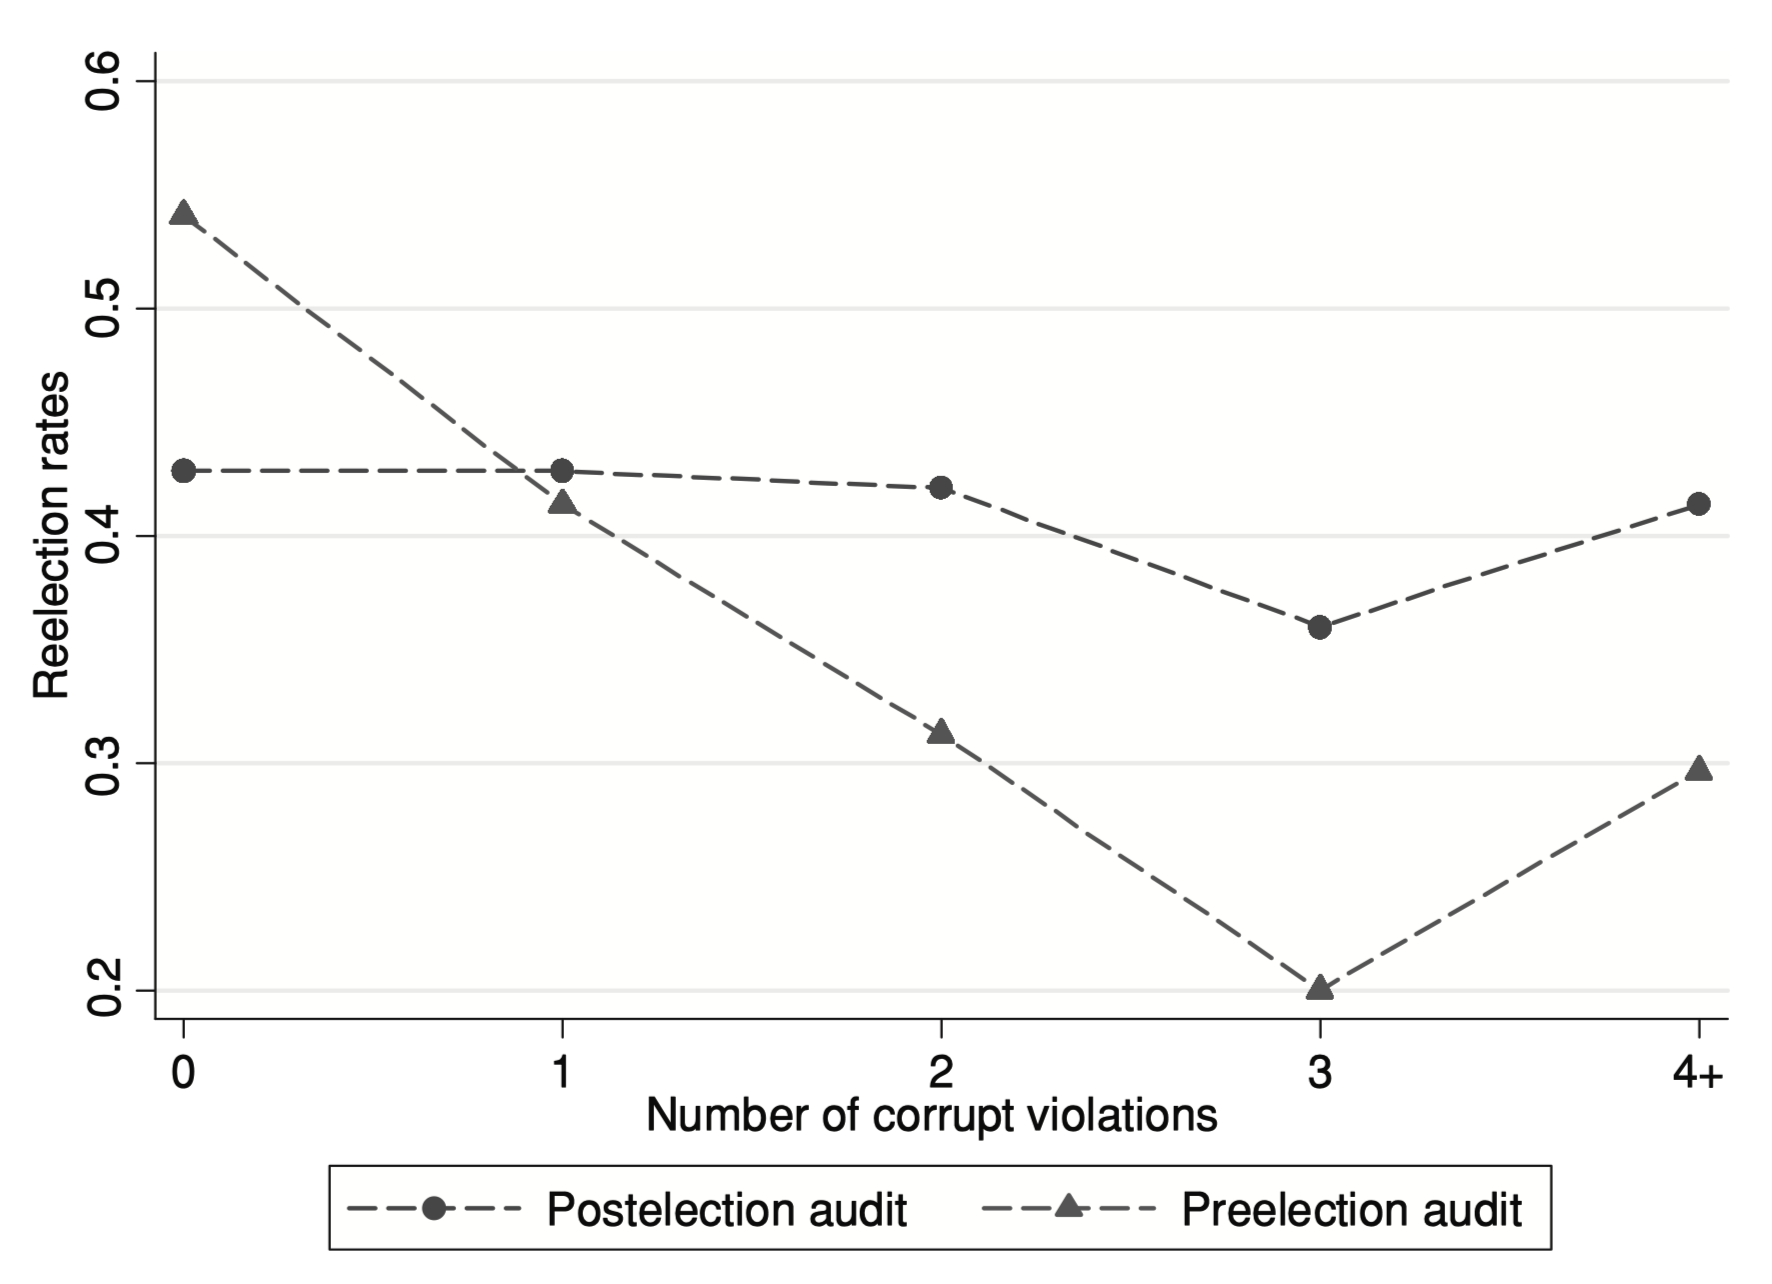
\includegraphics[height = 0.65 \textheight]{images/fig3.png}
        \caption{Descriptive evidence: Reelection Rates and Corruption Levels}
        \end{figure}
\end{frame}

\begin{frame}{Estimation II: Adding Voters' Prior Beliefs}

    \only<1>{
            \footnotesize
            \begin{align*}
                E_{ms} =& \alpha + \beta_0 C_{ms} + \beta_1 A_{ms} + \textcolor{orange}{\beta_2} \left(A_{ms}\times C_{ms}\right) + X_{ms}\gamma + \nu_s + \epsilon_{ms}
            \end{align*}
            }

    \begin{columns}

        \begin{column}{0.4\textwidth}
            \begin{figure}
            \centering
            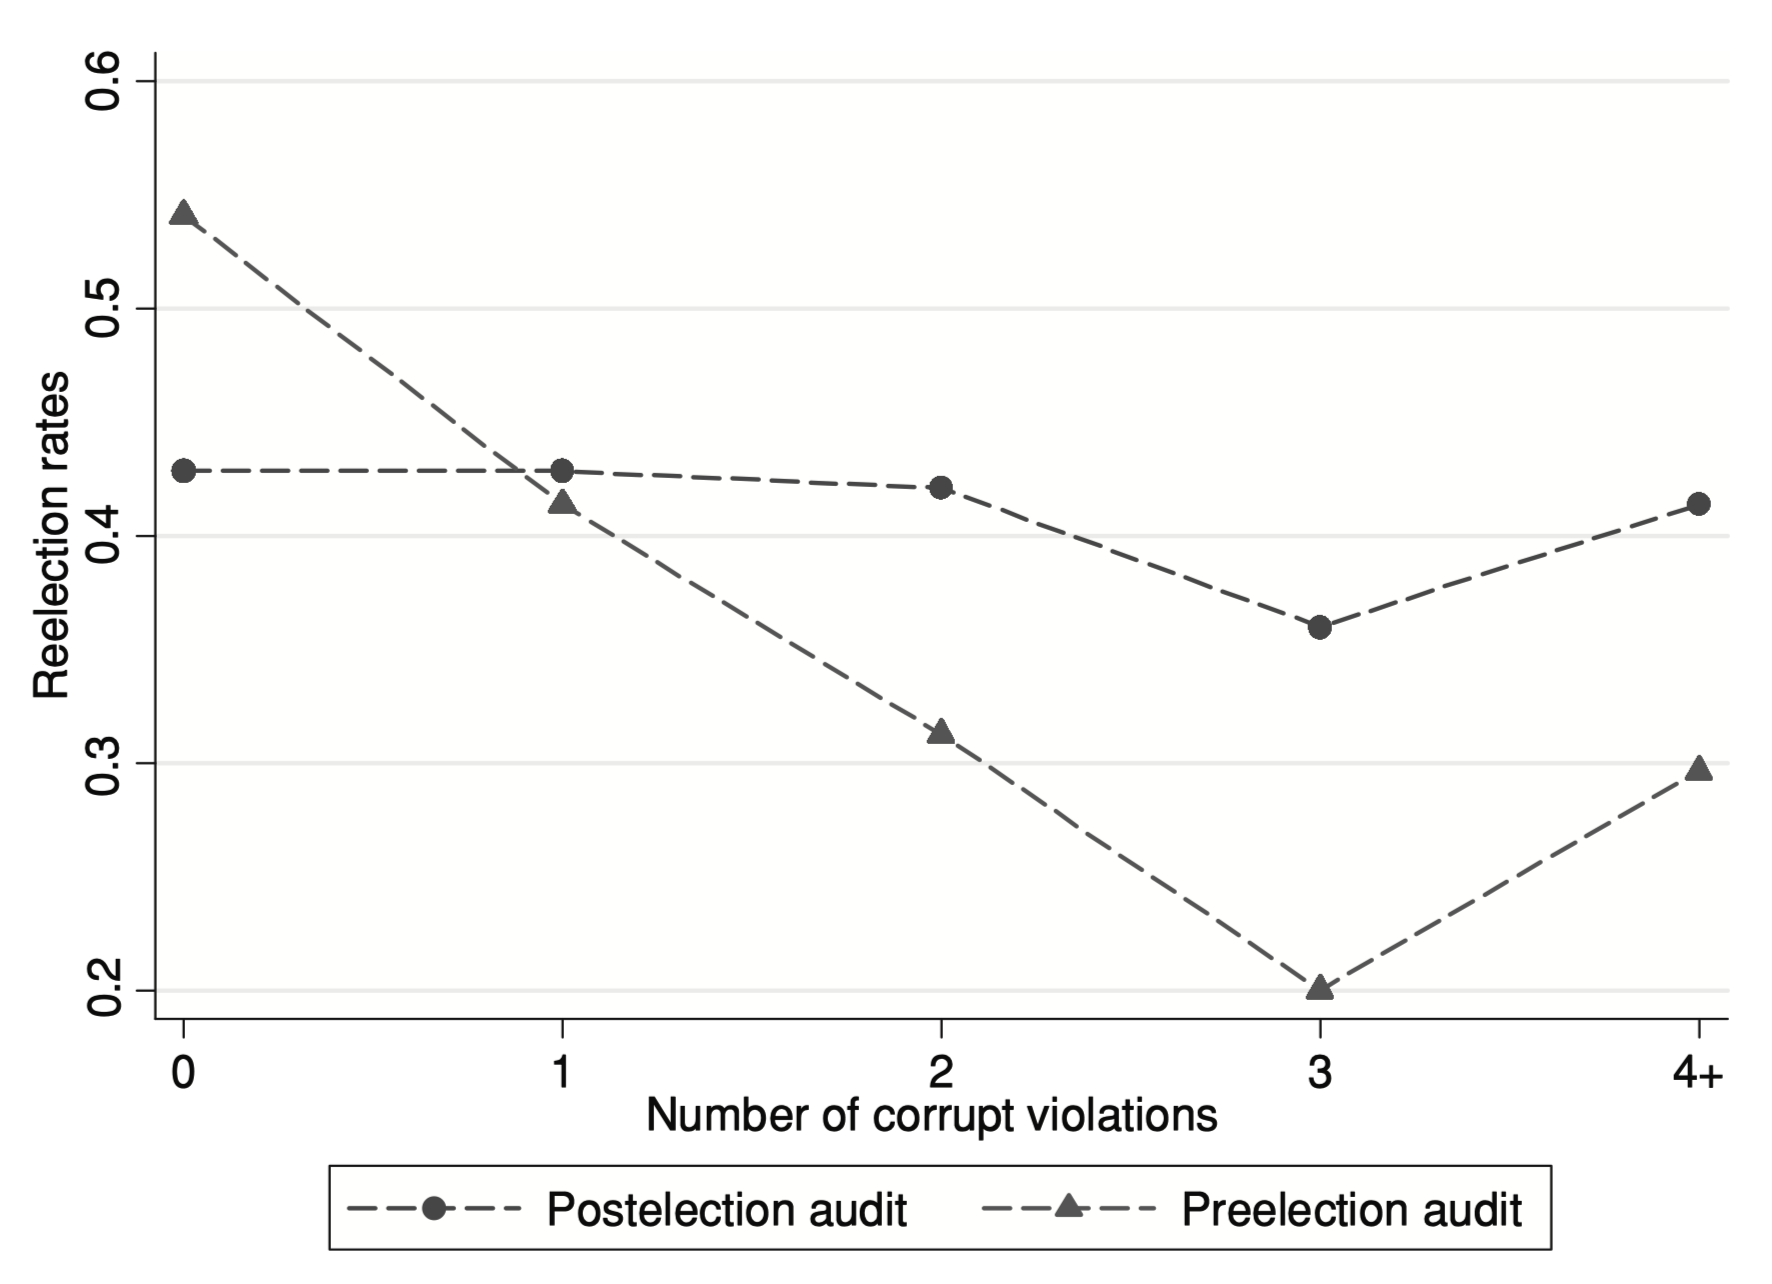
\includegraphics[height = 0.55 \textheight]{images/fig3.png}
            \end{figure}
        \end{column}

        \begin{column}{0.55\textwidth}

            \only<2->{
                \begin{table}[h!]
                    \footnotesize
                    \begin{center}
                        \label{tab:result2-1}
                        \begin{tabular}{lcc}
                        
                        \multicolumn{3}{c}{\color{orange}Linear}\\
                        & (1) & (2) \\
                        \hline
                        Preelection audit $\times$ & -0.038 & -0.038 \\
                         No. corruption violations & (0.035) & (0.035) \\
                         & \\
                         Observations & 373 & 373 \\
                         $R^2$ & 0.05 & 0.18\\
                         State FEs & Yes & Yes\\
                         Municipal controls & \textcolor{orange}{No} & \textcolor{orange}{Yes} \\
                         Mayoral controls & \textcolor{orange}{No} & \textcolor{orange}{Yes} 
                        \end{tabular}
                    \end{center}
                    \end{table}
            }
        
        \end{column}

    \end{columns}

\end{frame}

\begin{frame}{Estimation II: Adding Voters' Prior Beliefs}

    \begin{columns}

        \begin{column}{0.4\textwidth}
            \begin{figure}
            \centering
            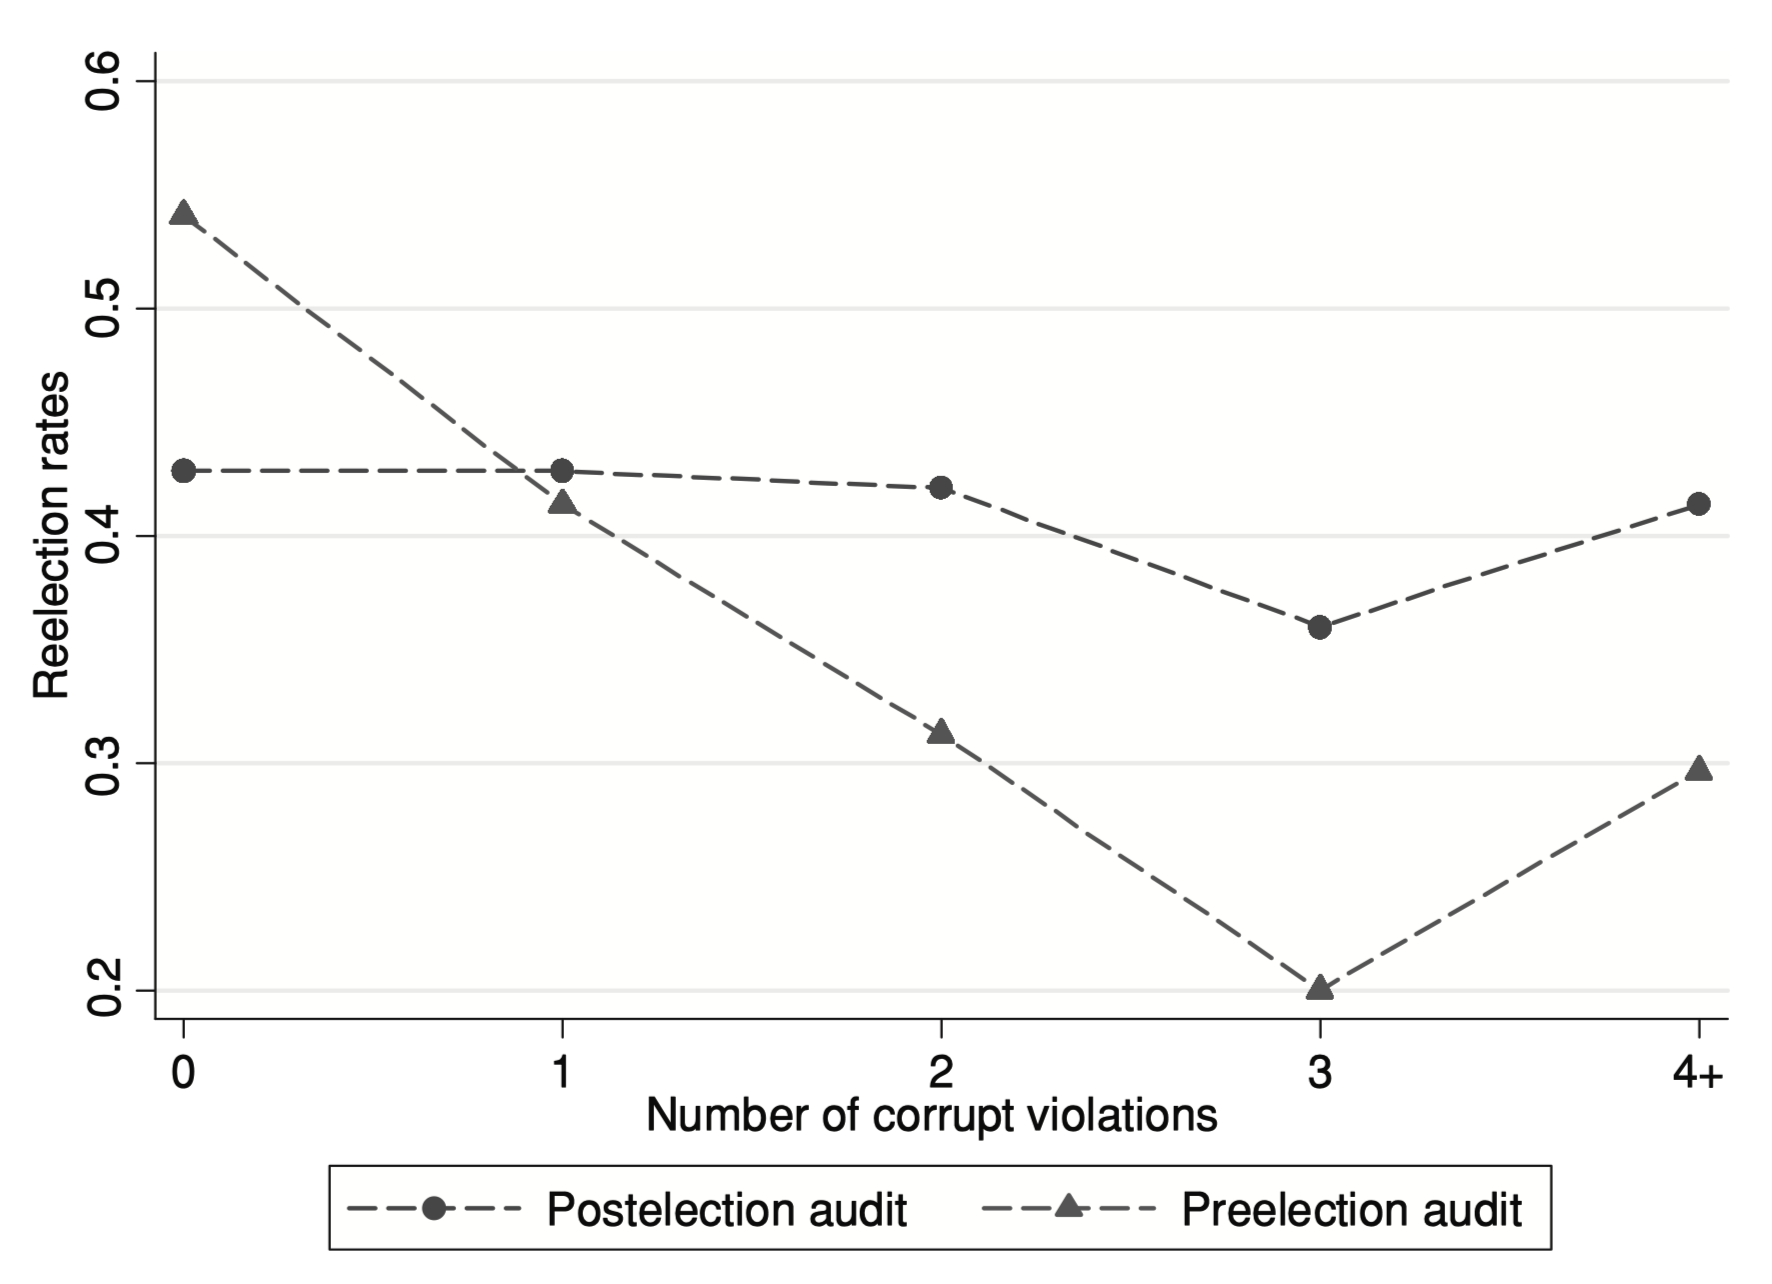
\includegraphics[height = 0.55 \textheight]{images/fig3.png}
            \end{figure}
        \end{column}

        \begin{column}{0.55\textwidth}

            \only<1->{
                \begin{table}[h!]
                    \tiny
                    \begin{center}
                        \label{tab:result2-2}
                        \begin{tabular}{lccc}
                        
                        \multicolumn{4}{c}{Different models}\\
                        \hline
                        & Linear & \textcolor<2>{orange}{Quadratic} & \textcolor<3>{orange}{Semiparametric} \\
                        & (2) & (3) & (4)\\
                        \hline
                        Preelection audit $\times$ & -0.038 & \textcolor<2>{orange}{-0.200$^*$} & \\
                         No. corruption violations & (0.035) & (0.090) & \\
                         Preelection audit $\times$ &  & \textcolor<2>{orange}{0.034$^*$} &\\
                         No. corruption violations$^2$ & & (0.017) &\\
                         
                         Preelection audit $\times$ &  & & 0.010\\
                         corruption = 0 & & & (0.156)\\
                         Preelection audit $\times$ &  & &  \textcolor<3>{orange}{-0.253$^+$}\\
                         corruption = 2 & & & (0.148)\\
                         Preelection audit $\times$ &  &  & \textcolor<3>{orange}{-0.321$^+$}\\
                         corruption = 3 & & & (0.192)\\
                         Preelection audit $\times$ &  &  & -0.159\\
                         corruption = 4 & & & (0.168)\\
                         & \\
                         $R^2$ & 0.18 & \textcolor<2>{orange}{0.19} & \textcolor<3>{orange}{0.22} \\
                         $F-$test ($p$-value) & & \textcolor<2>{orange}{0.089} & \textcolor<3>{orange}{0.192}
                        \end{tabular}
                    \end{center}
                    \end{table}
            
            }
        
        \end{column}

    \end{columns}

\end{frame}

\begin{frame}{Estimation II: Adding Voters' Prior Beliefs}

    \begin{columns}

        \begin{column}{0.4\textwidth}
            \begin{figure}
            \centering
            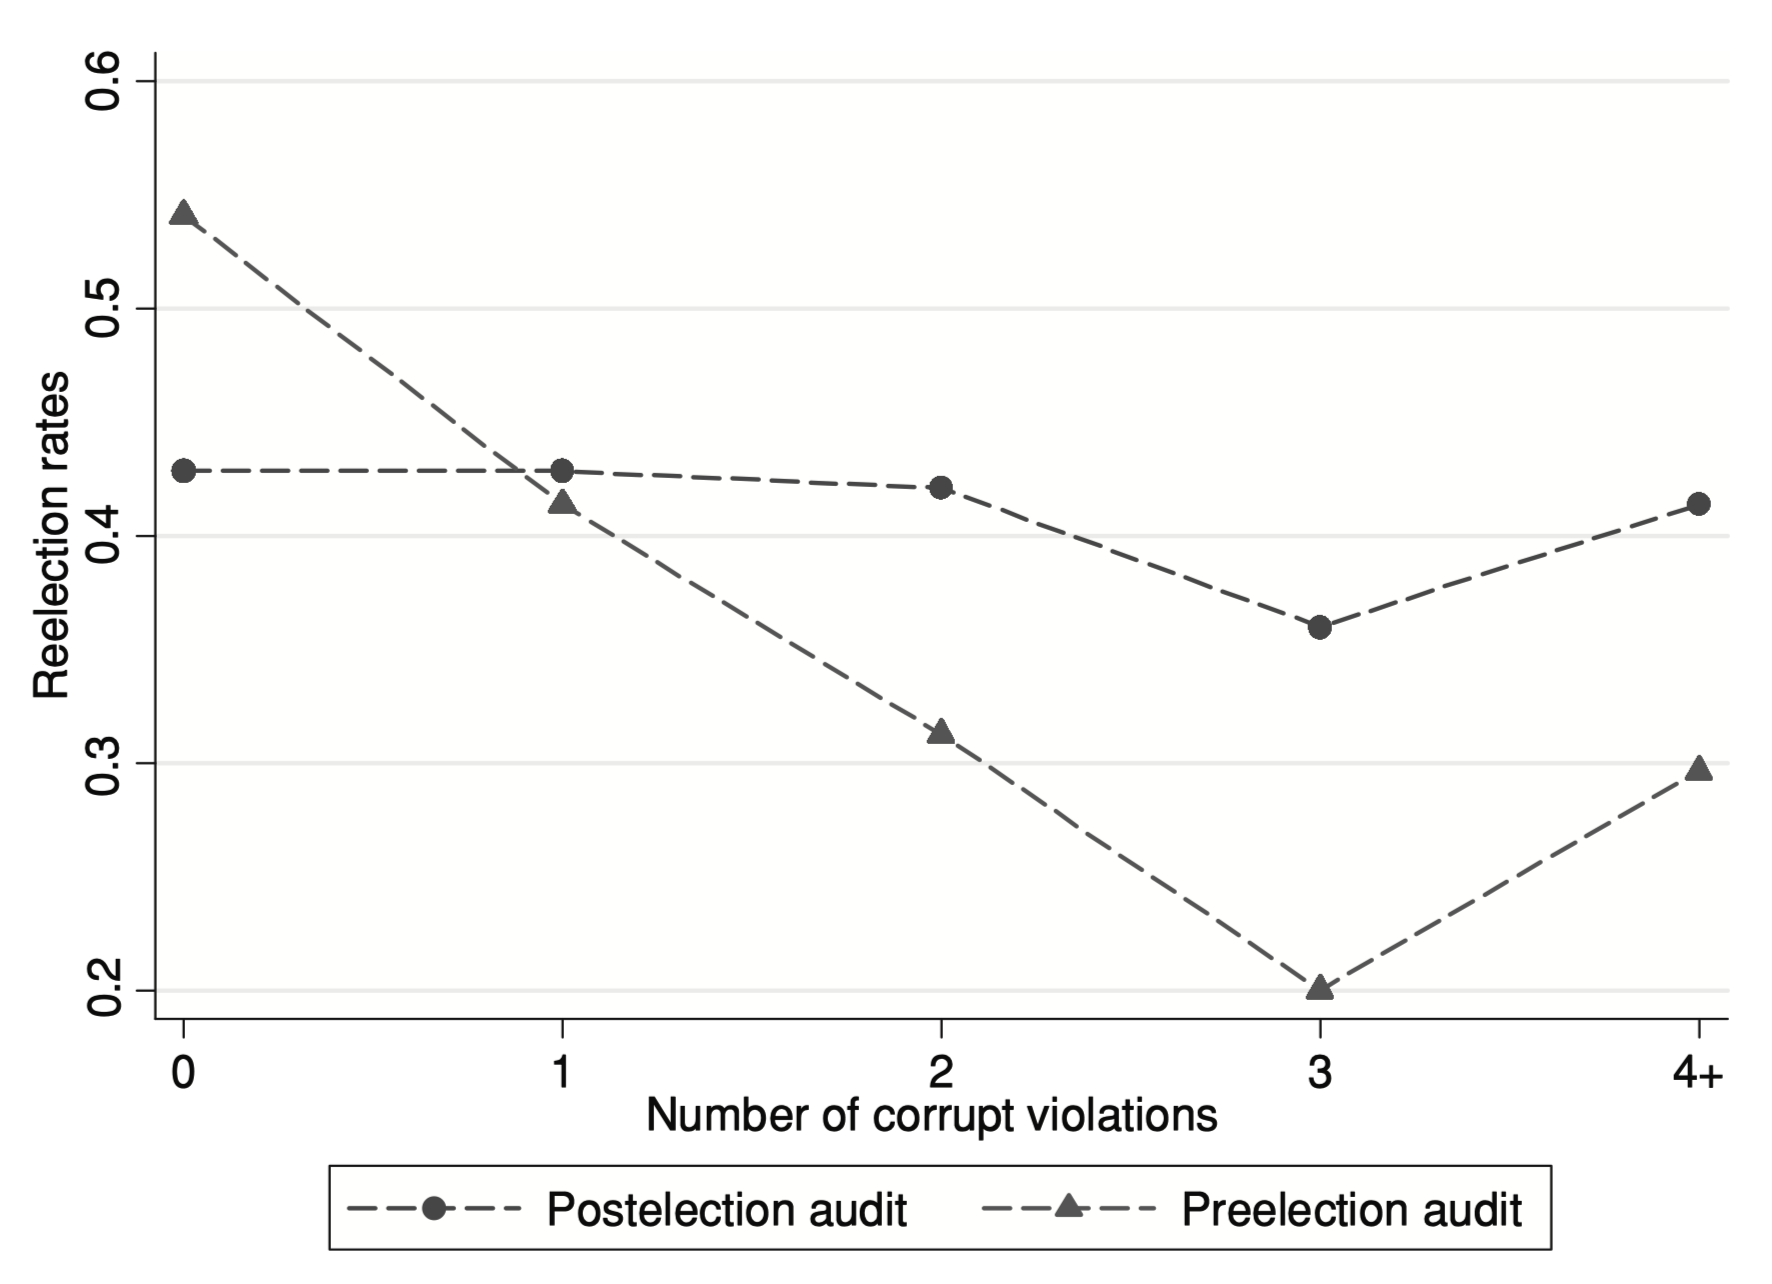
\includegraphics[height = 0.55 \textheight]{images/fig3.png}
            \end{figure}
        \end{column}

        \begin{column}{0.55\textwidth}

            \only<1->{
                \begin{table}[h!]
                    \tiny
                    \begin{center}
                        \label{tab:result2-3}
                        \begin{tabular}{lccc}
                        
                        \multicolumn{4}{c}{Different samples}\\
                        \hline
                        & Full & \textcolor<2>{orange}{Corruption$\leq$5} & \textcolor<3>{orange}{Corruption$\leq$4} \\
                        & (2) & (5) & (6)\\
                        \hline
                        Preelection audit $\times$ & -0.038 & \textcolor<2>{orange}{-0.070$^+$} & \textcolor<3>{orange}{-0.088$^*$} \\
                         No. corruption violations & (0.035) & (0.041) & (0.043)\\
                         & \\
                         Observations & 373 & \textcolor<2>{orange}{362} & \textcolor<3>{orange}{351} \\
                         $R^2$ & 0.18 & 0.19 & 0.20
                        \end{tabular}
                    \end{center}
                    \end{table} 
            
            }
        
        \end{column}

    \end{columns}

\end{frame}

\begin{frame}{Estimation II: Adding Voters' Prior Beliefs}

    \begin{columns}

        \begin{column}{0.4\textwidth}
            \begin{figure}
            \centering
            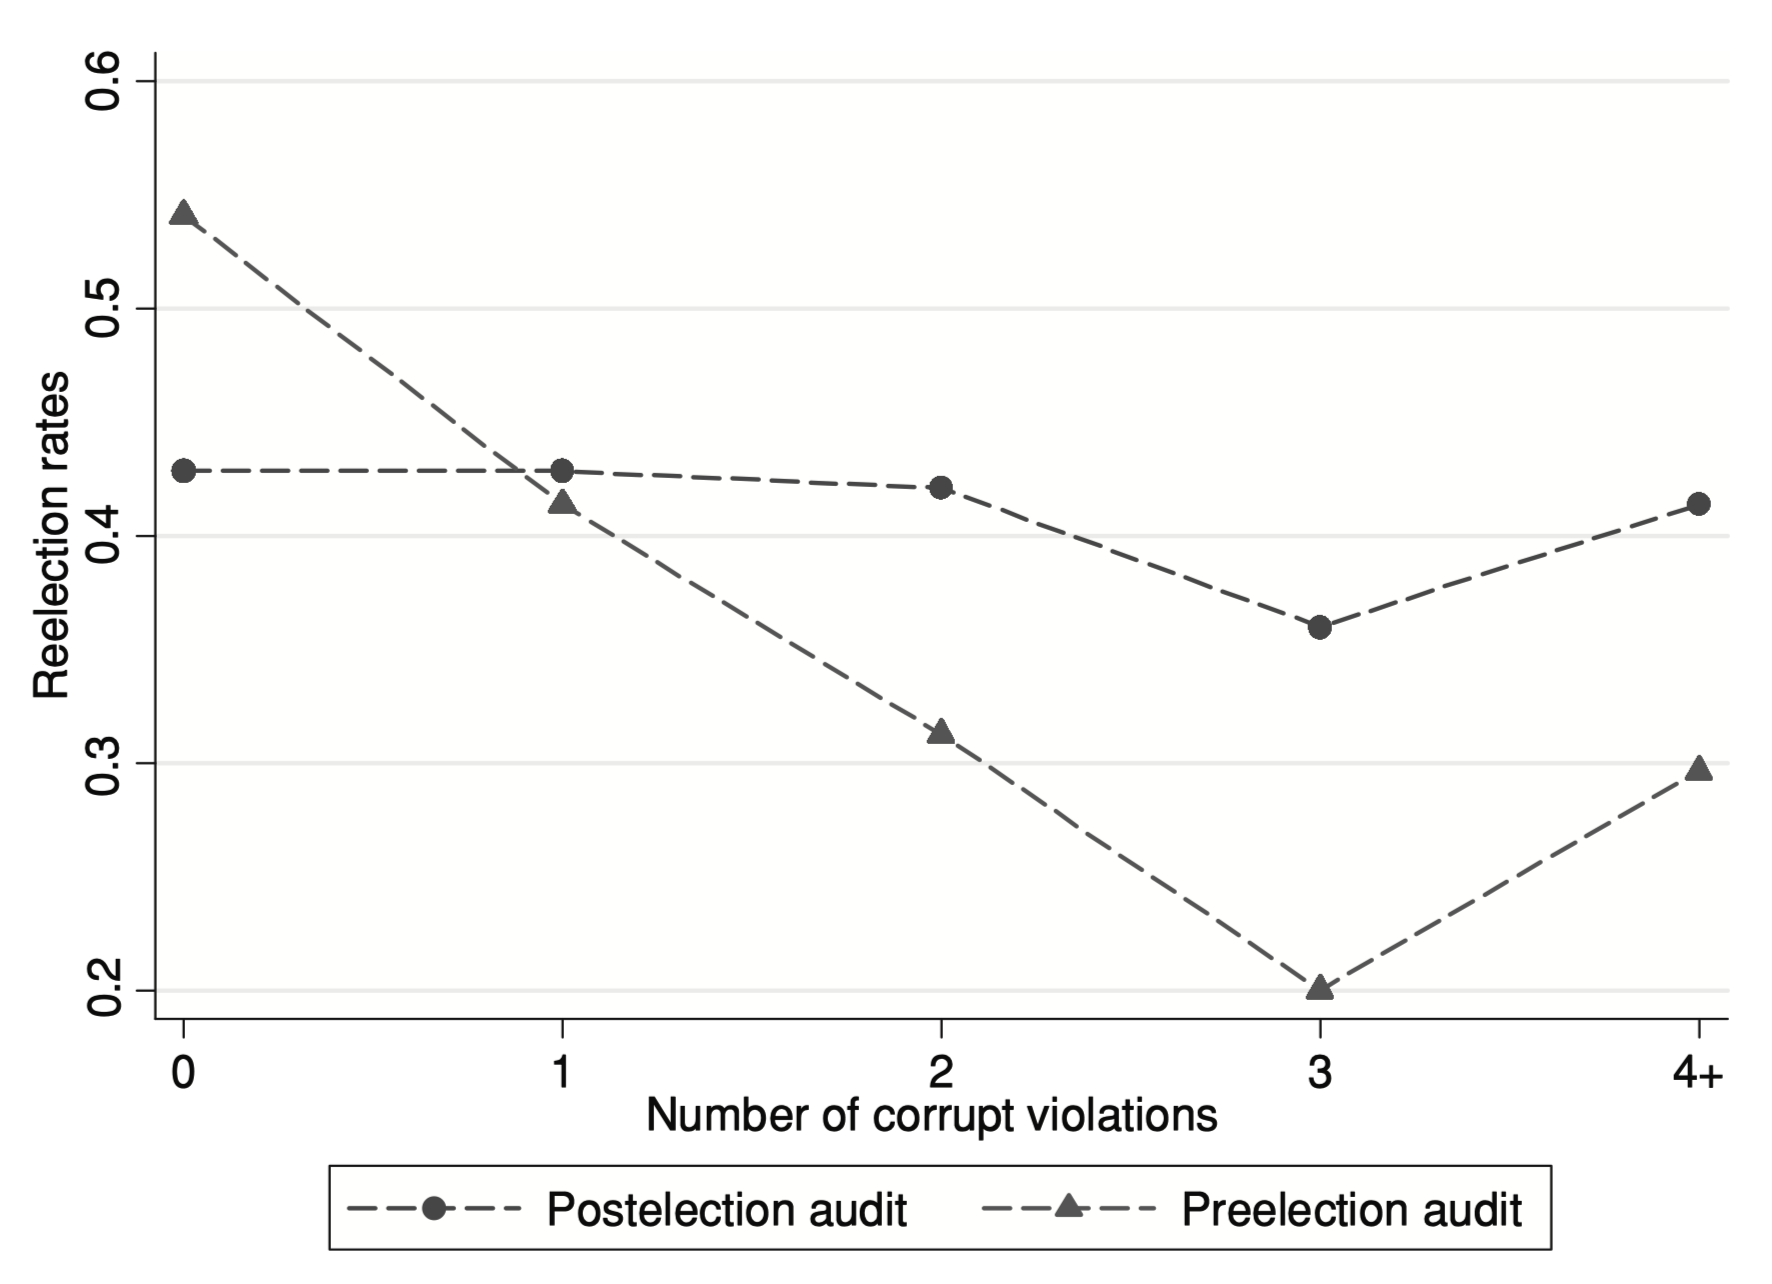
\includegraphics[height = 0.55 \textheight]{images/fig3.png}
            \end{figure}
        \end{column}

        \begin{column}{0.5\textwidth}

        \only<1->{
        \begin{block}{\small \textbf{Summary}}
        \footnotesize

            \only<1->{
                \begin{enumerate}
                    \item<2-> Model selection: The U-shape relationship is more likely driven by \textbf{\color{orange}noise}
                    \item<3-> Preferred specification: \textbf{\color{orange} Linear}, with the sub-sample of \textbf{\color{orange}Corruption$\leq$5} 
                    \item<4-> Estimation results: Marginal treatment effect per corruption violation is \textbf{\color{orange}-7\%} {\scriptsize (or \textbf{\color{orange}-16\%} of the 43\% control-group reelection rate)}.
                    \item<5-> Prior belief: Incumbents on average commit \textbf{\color{orange}1} corrupt violation 
                \end{enumerate}
            }
        \end{block}
        }

        \only<6>{\scriptsize
            \textbf{\color{orange}Question}: what about those extremely corrupted mayors?
        }
        
        \end{column}

    \end{columns}

\end{frame}


\begin{frame}{Estimation III: Adding the Presence of Local Media}
    \only<1->{
        \tiny
        \begin{align*}
        E_{ms} =& \alpha + \beta_0C_{ms} + \beta_1 A_{ms} + \textcolor<5>{orange}{\beta_2} M_{ms} + \textcolor<3>{orange}{\beta_3} \left(A_{ms}\times M_{ms}\right) + \beta_4\left(A_{ms}\times C_{ms}\right)\\
        & + \textcolor<4>{orange}{\beta_5} \left(M_{ms}\times C_{ms}\right) + \textcolor<2>{orange}{\beta_6} \left( A_{ms}\times C_{ms}\times M_{ms} \right) + X_{ms}\gamma+\nu_s +\epsilon_{ms}
        \end{align*}
    }

    \only<1->{
        \begin{table}[h!]
            \scriptsize
            \begin{center}
                \label{tab:result3-1}
                \begin{tabular}{lcccc}
                
                %\multicolumn{5}{c}{Dependent variable: Pr(reelection)}\\
                %\hline
                & & & & Demographics\\
                & Full & Corruption$\leq$5 & Demographics &  \& institutional  \\
                & (1) & (2) & (3) & (4) \\
                \hline
                 Preelection audit & -0.059 & -0.033 & 0.296 & 0.208 \\
                 No. corrupt violations & -0.034 & -0.013 & -0.13 & -0.069\\
                 No. radio stations & \textcolor<5>{orange}{-0.131$^*$} & \textcolor<5>{orange}{-0.150$^*$} & \textcolor<5>{orange}{-0.216$^{**}$} & \textcolor<5>{orange}{-0.253$^{**}$}\\
                 &\\
                 Preelection audit $\times$ No. radio stations & \textcolor<3>{orange}{0.229$^*$} & \textcolor<3>{orange}{0.271$^{**}$} & \textcolor<3>{orange}{0.356$^{**}$} & \textcolor<3>{orange}{0.449$^{**}$} \\
                 Preelection audit $\times$ No. corrupt violations & 0.007 & -0.018 & -0.236 & -0.412 \\
                 No. radio stations $\times$ No. corrupt violations & \textcolor<4>{orange}{0.050$^{+}$} & \textcolor<4>{orange}{0.058$^*$} & \textcolor<4>{orange}{0.082$^{**}$} &\textcolor<4>{orange}{0.09$^{**}$}\\
                 &\\
                 Triple interaction & \textcolor<2>{orange}{-0.118$^{**}$} & \textcolor<2>{orange}{-0.157$^*$} & \textcolor<2>{orange}{-0.185$^{**}$} & \textcolor<2>{orange}{-0.238$^{**}$}\\
                 &\\
                 $R^2$ & 0.20 &0.21 & 0.24 & 0.28
                \end{tabular}
            \end{center}
            \end{table}
    }

    
\end{frame}

\begin{frame}{Estimation III: Adding the Presence of Local Media}

    \begin{columns}

        \begin{column}{0.5\textwidth}
            \begin{figure}
            \centering
            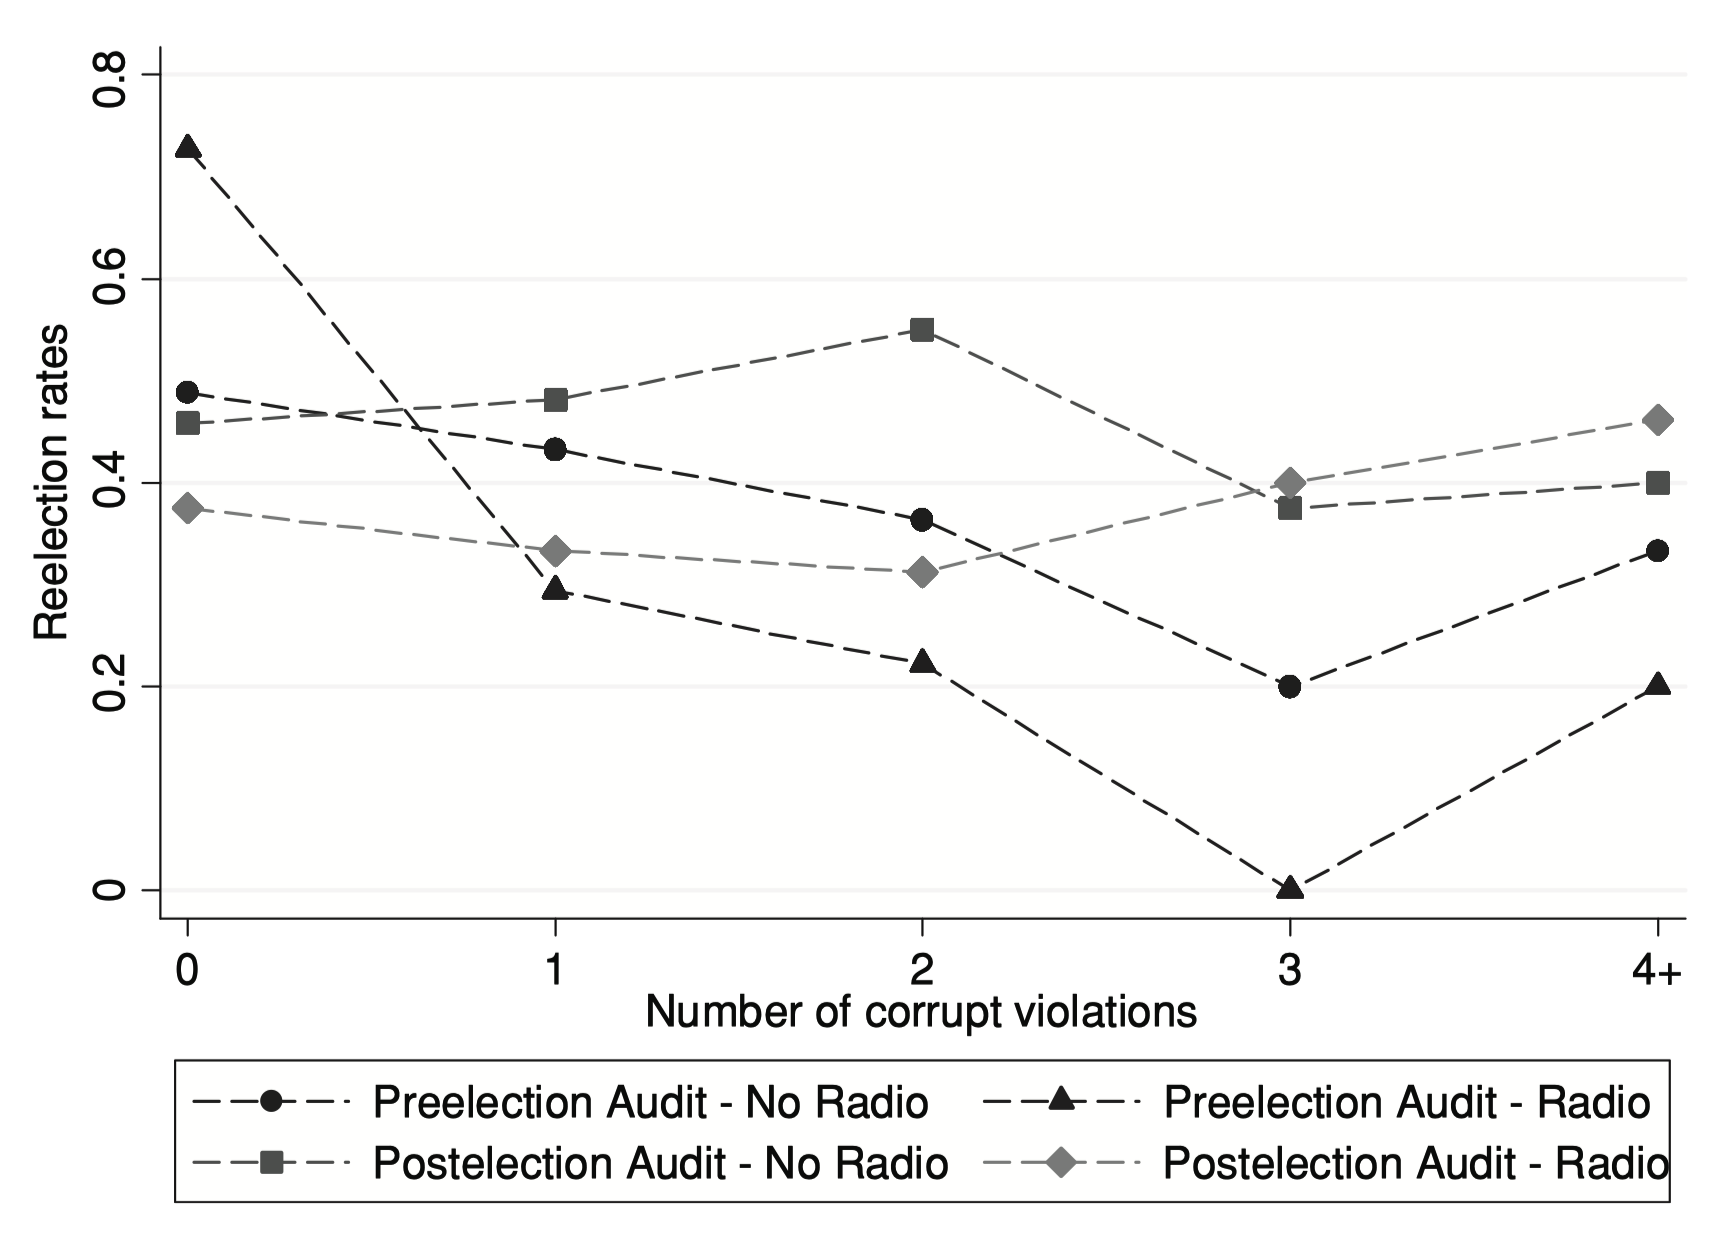
\includegraphics[height = 0.65 \textheight]{images/fig4.png}
            \end{figure}
        \end{column}

        \begin{column}{0.5\textwidth}

            \only<1->{
                \scriptsize
                \begin{align*}
                E_{ms} = & \alpha + \beta_0C_{ms} + \beta_1 A_{ms} + \textcolor{orange}{\beta_2} M_{ms} \\
                & + \textcolor{orange}{\beta_3} \left(A_{ms}\times M_{ms}\right) + \textcolor{orange}{\beta_5}\left(M_{ms}\times C_{ms}\right)\\
                & + \beta_4\left(A_{ms}\times C_{ms}\right) \\
                & + \textcolor{orange}{\beta_6} \left( A_{ms}\times C_{ms}\times M_{ms} \right) + X_{ms}\gamma+\nu_s +\epsilon_{ms}
                \end{align*}
            }

            \only<2->{
                \begin{itemize}
                    \item<2-> \textcolor{orange}{$\beta_6<0$}
                    \item<3-> \textcolor{orange}{$\beta_5>0$}, $\beta_4=0$, \textcolor{orange}{$\beta_3>0$}
                    \item<4-> \textcolor{orange}{$\beta_2<0$}, $\beta_1=0$, $\beta_0=0$ 
                \end{itemize}
            }

        
        \end{column}

    \end{columns}

\end{frame}